\documentclass[letterpaper,12pt,notitlepage]{report}
\usepackage{graphicx,amssymb,amstext,amsmath,geometry}
\usepackage{color,rotating}
\usepackage{tikz}
\usetikzlibrary{positioning,shapes,shadows,arrows}
\usepackage{pdflscape,caption}

\newcommand\etc{\textsl{etc}}
\newcommand\eg{\textsl{eg.}\ }
\newcommand\etal{\textsl{et al.}}
\newcommand\Quote[1]{\lq\textsl{#1}\rq}
\newcommand\fr[2]{{\textstyle\frac{#1}{#2}}}
\newcommand\miktex{\textsl{MikTeX}}
\newcommand\comp{\textsl{The Companion}}
\newcommand\nss{\textsl{Not so Short}}

\makeatletter
\newcommand*{\toccontents}{\@starttoc{toc}}
\makeatother

\begin{document}
\leftmargin 1.0cm
\rightmargin 0.0cm
\topmargin -2.0cm
\textwidth 16.0cm
\textheight 23.0cm
\oddsidemargin 0.5cm

\begin{center}
\thispagestyle{empty}
{\large {\bf GRIFFIN Data Format Specification}}\\
Compiled by Adam Garnsworthy, May 2015
\end{center}

\noindent The GRIFFIN data acquisition system runs under the MIDAS Data Acquisition system in order to record the data from the GRIFFIN HPGe spectrometer for decay spectroscopy experiments at TRIUMF-ISAC.\\

%\tableofcontents
\toccontents

\chapter{Introduction}

\section{Binary Counting Definition}

The bits in the words in this document are counted from 0 to 7 in each byte. There-
fore a 4-byte, 32 bit word contains bits from 0 to 31.\\

\noindent
An example of how the bits in a 16-bit, 2-byte word are counted in this document:\\

\begin{tabular}{l|cccc|cccc|cccc|cccc|}
Bit Number: & 15 & 14 & 13 & 12 & 11 & 10 & 09 & 08 & 07 & 06 & 05 & 04 & 03 & 02 & 01 & 00\\
Bit Weight: & \multicolumn{4}{l}{32,768} & \multicolumn{4}{|l}{2,048} &\multicolumn{4}{|l}{128} &\multicolumn{4}{|l|}{8}\\
\end{tabular}\\

\chapter{GRIF-16}

\section{Event Format and Size}

Detectors counting at a high rate will register multiple hits during a fixed evaluation period. In order to take advantage of higher counting rates, it is therefore essential to handle these pile-up events and recover the energies and times for every interaction in the detector. A method for extracting these energies and times is shown in figure \ref{pileup} which involves splitting the integration window of size, K, into multiple windows, K1, K2 etc. The event can also be flagged and the waveform output for evaluation offline.

\begin{figure}[h]
\centering
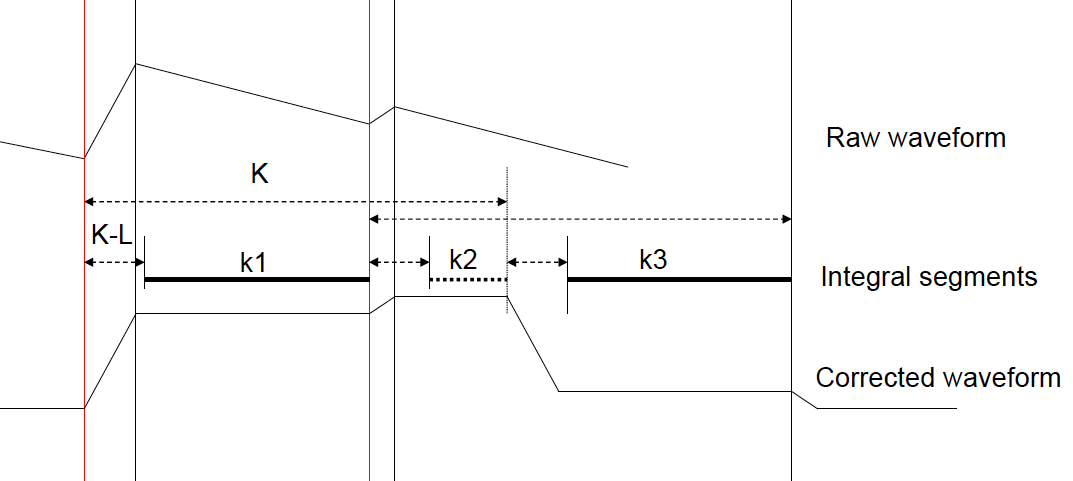
\includegraphics[width=16cm]{./Pileup_Waveforms.png}
\caption{\label{pileup}Method for extracting energy and time for pile-up events in the firmware.}
\end{figure}

\noindent The event format for handling pileup events is of variable size and depends on the number of hits in the evaluation window, the maximum is 3 hits in one window. The format is based on 4-byte (32-bit) words shown in the following tables, the number of bits for each sub-word is indicated in brackets. Waveforms can also be included at 2 bytes per sample.\\

\newpage
\begin{landscape}
\begin{table}
\caption{GRIFFIN GRIF-16 Event Format written to disk:}
\begin{tabular*}{\textwidth}{p{0.7cm}|p{2.7cm}|p{2.7cm}|p{2.7cm}|p{2.7cm}|p{2.7cm}|p{2.7cm}|c}
\cline{2-7}
I & Packet Type (4) {\bf 0x8} & Pile-Up Type (2) & Data Type (3) & Num. Filter Patterns (3) & Address (16) & Det. Type (4) & 4~bytes\\
\cline{2-7}
II & Fixed 00 (2) & \multicolumn{2}{c|}{Master Filter Patterns Passed (14)} & \multicolumn{3}{c|}{PPG Pattern (16)} & 4~bytes\\
\cline{2-7}
III & Fixed 0 (1) & \multicolumn{5}{c|}{Master Filter ID (31)} & 4~bytes\\
\cline{2-7}
IV & Packet Type (4) {\bf 0x9} & \multicolumn{5}{c|}{Channel Trigger ID (28)} & 4~bytes\\
\cline{2-7}
V & Packet Type (4) {\bf 0xa} & \multicolumn{5}{c|}{Time Stamp low bits (28)} & 4~bytes\\
\cline{2-7}
VI & Packet Type (4) {\bf 0xb} & \multicolumn{2}{c|}{Deadtime (14)} & \multicolumn{3}{c|}{Time Stamp high bits (14)} & 4~bytes\\
\cline{2-7}
VIa & Packet Type (4) {\bf 0xd} & \multicolumn{5}{c|}{Network Packet ID (28)} & 4~bytes\\
\cline{2-7}
VIb & Packet Type (4) {\bf 0xc} & \multicolumn{5}{c|}{Waveform Sample (28)} & 4~bytes\\
\cline{2-7}
VII & Fixed 0 (1) & Upper K1 bits (5) & \multicolumn{4}{c|}{K1 Pulse Height (26)} & 4~bytes\\
\cline{2-7}
VIII & Fixed 0 (1) & Lower K1 bits (5) & \multicolumn{4}{c|}{K1 Amplitude-Corrected Timing (26)} & 4~bytes\\
\cline{2-7}
IX & Fixed 0 (1) & Upper K2 bits (5) & \multicolumn{4}{c|}{K2 Pulse Height (26)} & 4~bytes\\
\cline{2-7}
X & Fixed 0 (1) & Lower K2 bits (5) & \multicolumn{4}{c|}{K2 Amplitude-Corrected Timing (26)} & 4~bytes\\
\cline{2-7}
XI & Fixed 0 (1) & Upper K3 bits (5) & \multicolumn{4}{c|}{K3 Pulse Height (26)} & 4~bytes\\
\cline{2-7}
XII & Fixed 0 (1) & Lower K3 bits (5) & \multicolumn{4}{c|}{K3 Amplitude-Corrected Timing (26)} & 4~bytes\\
\cline{2-7}
XIII & Packet Type (4) {\bf 0xe} & \multicolumn{2}{c|}{Event Trailer (10)} & \multicolumn{3}{c|}{Event Trailer - Repeated Time Stamp low bits (14)} & 4~bytes\\
\cline{2-7}
\multicolumn{5}{r}{Total one hit} & \multicolumn{2}{c}{9 words I-VIII+XIII:} & 36 bytes\\
\multicolumn{5}{r}{Total two hits} & \multicolumn{2}{c}{ 11 words I-X+XIII:} & 44 bytes\\
\multicolumn{5}{r}{Total three hits} & \multicolumn{2}{c}{ 13 words I-XIII:} & 52 bytes\\
\end{tabular*}
\end{table}
\end{landscape}

%%%%%%%%%%%%%%%%%%%%%%%%%%%%%%%%%%
\section{Pile-Up Type}
The Pile-Up Type indicates how many hits were recorded within the evaluation window, with the maximum being 3 hits in one window. The Pile-Up Type is provided in word I as bits 18-20 (2 bits).\\
Example of identifying a Header word type:\\

\begin{tabular}{ccccccccc}
Word I &  & Mask & & Shift & & Hex result & & Decimal result\\
0x8074A998 & \& & 0xF0000000 & $>>$ & 28 & = & 0x8 & = & 8\\  %change here
\end{tabular}\\

\noindent 
Example of extracting the Pile-Up Type:\\

\begin{tabular}{ccccccccc}
Word I &  & Mask & & Shift & & Hex result & & Decimal result\\
0x80007C80 & \& & 0x0C000000 & $>>$ & 26 & = & 0x0 & = & 0 (1 Hit)\\  %change here
0x84007C80 & \& & 0x0C000000 & $>>$ & 26 & = & 0x1 & = & 1 (2 Hit)\\  %change here
0x88007C80 & \& & 0x0C000000 & $>>$ & 26 & = & 0x2 & = & 2 (3 Hits)\\  %change here
0x8C007C80 & \& & 0x0C000000 & $>>$ & 26 & = & 0x3 & = & 3 ($>$3 Hits = Bad)\\  %change here
\end{tabular}

%%%%%%%%%%%%%%%%%%%%%%%%%%%%%%%%%%%%%%%%%%%%%%%%%
\section{Data Type}
The Data Type indicates where the data was generated (GRIF-16, GRIF-4G, GRIF-C etc.) and is provided in word I as bits 23-25 (3 bits). The  packet type is identified in the 4 upper bits of word I as type 8.\\
Example of identifying a Header word type:\\

\begin{tabular}{ccccccccc}
Word I &  & Mask & & Shift & & Hex result & & Decimal result\\
0x8074A998 & \& & 0xF0000000 & $>>$ & 28 & = & 0x8 & = & 8\\
\end{tabular}\\

\noindent The Data Type number can be extracted as:\\

\begin{tabular}{ccccccccc}
Word I &  & Mask & & Shift & & Hex result & & Decimal result\\
0x80A4A998 & \& & 0x03800000 & $>>$ & 23 & = & 0x1 & = & 1 (GRIF-16)\\
0x8124A998 & \& & 0x03800000 & $>>$ & 23 & = & 0x2 & = & 2 (GRIF-4G)\\
0x81A4A998 & \& & 0x03800000 & $>>$ & 23 & = & 0x3 & = & 3 (GRIF-C Slave)\\
0x8234A998 & \& & 0x03800000 & $>>$ & 23 & = & 0x4 & = & 4 (GRIF-C Master)\\
\end{tabular}

%%%%%%%%%%%%%%%%%%%%%%%%%%%%%%%%%%%%%%%%%%%%%%%%%
\section{Number of Filter Patterns}
The Number of Filter Patterns which have been satisfied by this event fragment is provided in word I as bits 20-22 (3 bits). The packet type is identified in the 4 upper bits of word I as type 8.\\
Example of identifying a Header word type:\\

\begin{tabular}{ccccccccc}
Word I &  & Mask & & Shift & & Hex result & & Decimal result\\
0x8074A998 & \& & 0xF0000000 & $>>$ & 28 & = & 0x8 & = & 8\\
\end{tabular}\\

\noindent The number of filter patterns can be extracted as:\\

\begin{tabular}{ccccccccc}
Word I &  & Mask & & Shift & & Hex result & & Decimal result\\
0x8614A998 & \& & 0x00700000 & $>>$ & 20 & = & 0x1 & = & 1 (1 pattern word)\\
0x8624A998 & \& & 0x00700000 & $>>$ & 20 & = & 0x2 & = & 2 (2 pattern words)\\
0x8634A998 & \& & 0x00700000 & $>>$ & 20 & = & 0x3 & = & 3 (3 pattern words)\\
\end{tabular}

%%%%%%%%%%%%%%%%%%%%%%%%%%%%%%%%%%%%%%%%%%
\section{Address}
The Address is provided in word I as bits 4 to 19 (16 bits). This indicates which channel on which module has provided this event fragment.\\
Example of identifying a Header word type:\\

\begin{tabular}{ccccccccc}
Word I &  & Mask & & Shift & & Hex result & & Decimal result\\
0x8074A998 & \& & 0xF0000000 & $>>$ & 28 & = & 0x8 & = & 8\\
\end{tabular}\\

\noindent An example of unpacking the Address from the header word:\\
\begin{tabular}{ccccccccc}
Word I &  & Mask & & Shift & & Hex result & & Decimal result\\
0x82228280 & \& & 0x000FFFF0 & $>>$ & 4 & = & 0x0505 & = & 1285\\
\end{tabular}\\

\noindent The various properties with the Address word are as follows:\\

\begin{tabular}{cccl}
Property & Size & Values & Description\\
M & 4 bits & 0 to 15 & Input channel to Master or ID number of Slave\\
S & 4 bits & 0 to 15 & Input channel to Slave or ID number of Digitizer\\
C & 8 bits & 0 to 255 & Input channel to Digitizer\\
\end{tabular}\\

\noindent These properties can be extracted from this 16 bit word in the following way:\\

\begin{tabular}{ccccccccc}
Address &  & Mask & & Shift & & Hex result & & Decimal result\\
0x1405 & \& & 0x0000F000 & $>>$ & 12 & = & 0x01 & = & 1 (M)\\
0x1405 & \& & 0x00000F00 & $>>$ & 8 & = & 0x04 & = & 4 (S)\\
0x1405 & \& & 0x000000FF & $>>$ & 0 & = & 0x05 & = & 5 (C)\\
\end{tabular}

%%%%%%%%%%%%%
\section{Detector Type}
The Detector Type is provided in word I as bits 0 to 3 (4 bits). This indicates which detector type has generated this event fragment and is used primarily in master filter decisions.\\
Example of identifying a Header word type:\\

\begin{tabular}{ccccccccc}
Word I &  & Mask & & Shift & & Hex result & & Decimal result\\
0x8074A928 & \& & 0xF0000000 & $>>$ & 28 & = & 0x8 & = & 8\\
\end{tabular}\\

\noindent The Detector Type value can be extracted as:\\

\begin{tabular}{ccccccccc}
Word I &  & Mask & & Shift & & Hex result & & Decimal result\\
0x8074A900 & \& & 0x0000000F & $>>$ & 0 & = & 0x00 & = & 00 (HPGe Low Gain)\\
0x8074A902 & \& & 0x0000000F & $>>$ & 0 & = & 0x02 & = & 02 (SCEPTAR)\\
0x8074A905 & \& & 0x0000000F & $>>$ & 0 & = & 0x05 & = & 05 (Si(Li))\\
\end{tabular}\\

\noindent Here is a full list of GRIFFIN Detector Types:\\
\begin{tabular}{cccl}
{\bf ID} & {\bf Short Name} & {\bf Full Name} & {\bf Description}\\
00 & GRGa & Ge & 16 HPGe Clovers Low Gain\\
01 & GRGb & Ge & 16 HPGe Clovers High Gain\\
02 & SEP & Beta & 20 plastic scintillators (SCEPTAR)\\
03 & DAN & DANTE & 8 LaBr3 scintillators Energy signals\\
04 & DAT & DANTE & 8 LaBr3 scintillators TAC signals\\
05 & PAC & PACES & 5 SiLi for ICE\\
06 & DSC & DESCANT & 70 Scintillators for neutrons\\
07 & GRS & Suppressors & 16 sets of BGO for clovers\\
08 & DAS & Suppressors & 8 sets of BGO for DANTE\\
09 & SET & Beta & Zero-Degree scintillator (ZDS)\\
10 & DSC & DESCANT (Gamma) & Gamma identified by pulse shape\\
11 & DSC & DESCANT (Neutron) & Neutron identified by pulse shape\\
12 &  &  & Undefined\\
13 &  &  & Undefined\\
14 &  &  & Undefined\\
15 &  &  & Undefined\\
\end{tabular}

%%%%%%%%%%%%%%
\section{Master Filter ID}
The Master Filter ID is provided in word III as 31 bits. The Master Filter ID is an event counter which is reset at the start of a run and increments by 1 each time a new event master filter condition is passed in the master filter algorithm in the Master GRIF-C. The maximum value is 2147483649 above which the counter will wrap around.\\
Example of extracting the Master Filter ID:\\

\begin{tabular}{ccccccccc}
Word II &  & Mask & & Shift & & Hex result & & Decimal result\\
0x56007C84 & \& & 0x7FFFFFFF & $>>$ & 0 & = & 0x56007C84& = & 1442872452\\
\end{tabular}

%%%%%%%%%%%%%%
\section{Master Filter Pattern}
There are up to eight (more in the future) Filter Patterns which can be set and tested for every fragment. The Identifier(s) (1-8) of the Filter Pattern which was passed is provided in word II as bits 16 to 30 (14 bits). If multiple Filter conditions were passed by this fragment then there will be multiple Filter Patterns indicated in this word.\\
Example of extracting the Master Filter Pattern(s):\\

\begin{flushleft}
\begin{tabular}{ccccccccc}
Word III &  & Mask & & Shift & & Hex result & & Decimal result\\
0x00010F81 & \& & 0x7FFF0000 & $>>$ & 16 & = & 0x0001 & = & 1 (Only Filter 1 passed)\\
0x00050F81 & \& & 0x7FFF0000 & $>>$ & 16 & = & 0x0005 & = & 5 (Filters 1 and 3 passed)\\
0x00850F81 & \& & 0x7FFF0000 & $>>$ & 16 & = & 0x0085 & = & 133 (Filters 1, 3 and 8 passed)\\
\end{tabular}
\end{flushleft}

%%%%%%%%%%%%%%
\section{PPG Pattern}
The PPG Pattern is a recording of the Programable Pattern Generator status at the time that the threshold crossing occurred, and is provided in word II as bits 0 to 15 (16 bits). The pattern represents, for example, if the beam were being delivered or if it was blocked for decay counting etc.\\
Example of extracting the PPG Pattern:\\

\begin{tabular}{ccccccccc}
Word III &  & Mask & & Shift & & Hex result & & Decimal result\\
0x0F810F81 & \& & 0x0000FFFF & $>>$ & 0 & = & 0x00000F81 & = & 3969\\
\end{tabular}

%%%%%%%%%%%%%%
\section{Channel Trigger ID}
The Channel Trigger ID is provided in word IV as the 28 lower bits. The Channel Trigger ID is an event counter which is reset at the start of a run and increments by 1 each time a new threshold crossing occurs for this channel on the GRIF-16 or GRIF-4G. The word type is identified in the 4 upper bits as type 9.\\
Example of identifying the Channel Trigger ID word type:\\

\begin{tabular}{ccccccccc}
Word IV &  & Mask & & Shift & & Hex result & & Decimal result\\
0x900461FF & \& & 0xF0000000 & $>>$ & 28 & = & 0x9 & = & 9\\
\end{tabular}\\

\noindent The Channel Trigger ID number can wrap around if it becomes too large. The user should monitor the channel trigger id numbers which should increase throughout the run. The maximum value of channel trigger id is 268435455. If the number changes from very large to small then the counter has wrapped around, this should be tested at every event.

\noindent Example of unpacking the Channel Trigger ID:\\

\begin{tabular}{ccccccccc}
Word IV &  & Mask & & Shift & & Hex result & & Decimal result\\
0x900461FF & \& & 0x0FFFFFFF & $>>$ & 0 & = & 0x000461FF & = & 287231\\
\end{tabular}

%%%%%%%%%%%%%%
\section{Timestamp}
The timestamp is stored in two separate words as the lower 28 bits and 14 bits of the two words, word V and word VI respectively. Word V is the lower bits of the Timestamp and Word VI is the upper bits of the Timestamp. The type is identified in the 4 upper bits of both words as type 10 for the lower bits and 11 for the upper bits.\\
Example of identifying a Timestamp word type:\\

\begin{tabular}{ccccccccc}
Word V/VI &  & Mask & & Shift & & Hex result & & Decimal result\\
0xA074A998 & \& & 0xF0000000 & $>>$ & 28 & = & 0xA & = & 10 (lower bits)\\
0xB074A998 & \& & 0xF0000000 & $>>$ & 28 & = & 0xB & = & 11 (upper bits)\\
\end{tabular}\\

\noindent
An example of unpacking the Timestamp value:\\

\begin{tabular}{ccccccccr}
Word V/VI &  & Mask & & Shift & & Hex result & & Decimal result\\
0xA074A998 & \& & 0x0FFFFFFF & $>>$ & 0 & = & 0x0074A998 & = & 7645592\\
0xB0000005 & \& & 0x00003FFF & $>>$ & 0 & = & 0x00000005 & = & 5\\
\end{tabular}\\

\noindent
The upper and lower bits of the Timestamp can then be combined to make the full 42-bit timestamp. This is done in two steps by shifting the upper bits and then adding the lower bits using a bitwise or ($||$):\\

\begin{tabular}{ccccccr}
\multicolumn{3}{c}{Build Timestamp} & & Hex result & & Decimal result\\
0x00000005 & $<<$ & 28 & = & 0x05000000\\
0x05000000 & $||$ & 0x0074A998 & = & 0x0574A998 & = & 91531672\\
\end{tabular}\\

\noindent
The timestamp is in units of 10~nanoseconds and has a maximum value of 4,398,046,511,103. The timestamp will therefore reset either after 509 days or when the GRIF-C Master module is power cycled.\\

\noindent The 28 lower bits are also stored in the event trailer.

%%%%%%%%%%%%%%

\section{Deadtime}
There are two methods of determining the event-by-event deadtime of the system for precision measurements; firstly to operate at a fixed deadtime for every event, or secondly to measure and record the deadtime of each event. Both methods will be trialled and evaluated as part of the GRIFFIN DAQ development.\\

\noindent
The deadtime for each event is provided as bits 14-27 (14 bits) of word VII. The type is identified in the 4 upper bits as type 11.\\
Example of identifying a Deadtime word type:\\

\begin{tabular}{ccccccccc}
Word VII &  & Mask & & Shift & & Hex result & & Decimal result\\
0xB074A998 & \& & 0xF0000000 & $>>$ & 28 & = & 0xB & = & 11\\
\end{tabular}\\

\noindent
An example of unpacking the Deadtime value:\\

\begin{tabular}{ccccccccr}
Word VII &  & Mask & & Shift & & Hex result & & Decimal result\\
0xC074A998 & \& & 0x0FFFFC000 & $>>$ & 14 & = & 0x0074A998 & = & 7645592\\
\end{tabular}\\

The deadtime is in units of 10~ns and the maximum value is 16,383 representing 162.383 microseconds of deadtime for this event readout.

%%%%%%%%%%%%%%
\section{Network Packet ID}
The Network Packet ID is currently provided in word VIa as the 28 lower bits. The Network Packet ID is an event counter which is reset at the start of a run and increments by 1 each time a new event is dispatched by the GRIF-C master. The word type is identified in the 4 upper bits as type 9.\\
Example of identifying the Network Packet ID word type:\\

\begin{tabular}{ccccccccc}
Word VIa &  & Mask & & Shift & & Hex result & & Decimal result\\
0xD00461FF & \& & 0xF0000000 & $>>$ & 28 & = & 0xD & = & 13\\
\end{tabular}\\

\noindent The Network Packet ID number can wrap around if it becomes too large. The user should monitor the Network Packet id numbers which should increase throughout the run. The maximum value of Network Packet ID is 268435455. If the number changes from very large to small then the counter has wrapped around, this should be tested at every event.

\noindent Example of unpacking the Network Packet ID:\\

\begin{tabular}{ccccccccc}
Word VIa &  & Mask & & Shift & & Hex result & & Decimal result\\
0xD00461FF & \& & 0x0FFFFFFF & $>>$ & 0 & = & 0x000461FF & = & 287231\\
\end{tabular}

%%%%%%%%%%%%%%
\section{Waveform Data}
The Waveform Data is provided in multiple words, the number of which depends on the waveform length. These words are inserted into the event between words VI and VII. Waveform data words can be identified by their type which is in the 4 upper bits of each words as type C.

\begin{tabular}{ccccccccc}
Word &  & Mask & & Shift & & Hex result & & Decimal result\\
0xC57715CC & \& & 0xF0000000 & $>>$ & 28 & = & 0xC & = & 12\\
\end{tabular}\\

The Waveform Data values are in units of ADC bins.

%%%%%%%%%%%%%%

\section{K Values}
The 10 bits of the K value are provided in words VII and VIII as bits 26-30.\\
Example of extracting the K value:\\

\begin{tabular}{ccccccccc}
Word VII/VIII &  & Mask & & Shift & & Hex result & & Decimal result\\
0x2074A998 & \& & 0x7C000000 & $>>$ & 26 & = & 0x08 & = & 8\\
0x5874A998 & \& & 0x7C000000 & $>>$ & 26 & = & 0x16 & = & 22\\
\end{tabular}\\
The upper and lower bits of the K value can then be combined to make the full K value. This is done in two steps by shifting the upper bits and adding the lower bits:\\

\begin{tabular}{ccccccr}
\multicolumn{3}{c}{Build K Value} & & Hex result & & Decimal result\\
0x08 & $<<$ & 5 & = & 0x100\\
0x100 & $||$ & 0x16 & = & 0x116 & = & 278\\
\end{tabular}

%%%%%%%%%%%%%
\section{Pulse Height Signal}
The pulse height signal is provided in word VII as the 26 lower bits, which represent Pulse height 1. The maximum value is 67108863 and is in units of ADC channels.\\

\noindent
Two examples of unpacking the Pulse Height value:\\

\begin{tabular}{ccccccccc}
Word VII &  & Mask & & Shift & & Hex result & & Decimal result\\
0x680001FF & \& & 0x03FFFFFF & $>>$ & 0 & = & 0x000001FF & = & 511\\
0x680005B5 & \& & 0x03FFFFFF & $>>$ & 0 & = & 0x000005B5 & = & 1461\\
\end{tabular}\\

\noindent
For pile-up events the charge value of the secondary interactions are given in words X and XII.

%%%%%%%%%%%%%
\section{Amplitude-Corrected Timing Signal}
The timing from a Amplitude-Corrected Timing algorithm is provided in word VIII as the 26 lower bits. The maximum value is 67108863 and is in units of 10 nanoseconds.

\noindent
Two examples of unpacking the Amplitude-Corrected timing value:\\

\begin{tabular}{ccccccccc}
Word VIII &  & Mask & & Shift & & Hex result & & Decimal result\\
0x78000052 & \& & 0x03FFFFFF & $>>$ & 0 & = & 0x00000052 & = & 82\\
0x780000F6 & \& & 0x03FFFFFF & $>>$ & 0 & = & 0x000000F6 & = & 246\\
\end{tabular}\\

\noindent
For pile-up events the Amplitude-Corrected timing values of the secondary interactions are given in words VIII and XII.

%%%%%%%%%%%%%%
\section{Event Trailer}
The Event Trailer is provided in word XIII and it indicates the end of the event fragment. The type is identified in the 4 upper bits as type 14.\\
Example of identifying the Event Trailer word type:\\

\begin{tabular}{ccccccccc}
Word XIII &  & Mask & & Shift & & Hex result & & Decimal result\\
0xEEEEEEEE & \& & 0xF0000000 & $>>$ & 28 & = & 0xE & = & 14\\
\end{tabular}

\noindent
The 14 lower bits of the timestamp is repeated in the event trailer. This can be used as an additional check to ensure the event is not corrupted. An example of unpacking the lower bits of the Timestamp value from the Event Trailer word:\\

\begin{tabular}{ccccccccr}
Word XIII &  & Mask & & Shift & & Hex result & & Decimal result\\
0xE074A998 & \& & 0x0003FFFF & $>>$ & 0 & = & 0x0000A998 & = & 43416\\
\end{tabular}

%%%%%%%%%%%%%%%%%%%%%%%%%%%%%%%%%%%%%%%%%%%%%%%%%
%%%%%%%%%%%%%%%%%%%%%%%%%%%%%%%%%%%%%%%%%%%%%%%%%
%%%%%%%%%%%%%%%%%%%%%%%%%%%%%%%%%%%%%%%%%%%%%%%%%
%%%%%%%%%%%%%%%%%%%%%%%%%%%%%%%%%%%%%%%%%%%%%%%%%
%%%%%%%%%%%%%%%%%%%%%%%%%%%%%%%%%%%%%%%%%%%%%%%%%
%%%%%%%%%%%%%%%%%%%%%%%%%%%%%%%%%%%%%%%%%%%%%%%%%
\chapter{GRIF-4G}

\noindent
The format from this digitizer will be similar to that of the GRIF-16 but additional information may be provided associated with DESCANT detectors. This information will include output from additional signal-processing modules such as a neutron-gamma discrimination algorithm.\\

\newpage
\begin{landscape}
\begin{table}
\caption{GRIFFIN GRIF-4G Event Format written to disk:}
\begin{tabular*}{\textwidth}{p{0.7cm}|p{2.7cm}|p{2.7cm}|p{2.7cm}|p{2.7cm}|p{2.7cm}|p{2.7cm}|c}
\cline{2-7}
I & Packet Type (4) {\bf 0x8} & Pile-Up Type (2) & Data Type (3) & Num. Filter Patterns (3) & Address (16) & Det. Type (4) & 4~bytes\\
\cline{2-7}
II & Fixed 00 (2) & \multicolumn{2}{c|}{Master Filter Patterns Passed (14)} & \multicolumn{3}{c|}{PPG Pattern (16)} & 4~bytes\\
\cline{2-7}
III & Fixed 0 (1) & \multicolumn{5}{c|}{Master Filter ID (31)} & 4~bytes\\
\cline{2-7}
IV & Packet Type (4) {\bf 0x9} & \multicolumn{5}{c|}{Channel Trigger ID (28)} & 4~bytes\\
\cline{2-7}
V & Packet Type (4) {\bf 0xa} & \multicolumn{5}{c|}{Time Stamp low bits (28)} & 4~bytes\\
\cline{2-7}
VI & Packet Type (4) {\bf 0xb} & \multicolumn{2}{c|}{Deadtime (14)} & \multicolumn{3}{c|}{Time Stamp high bits (14)} & 4~bytes\\
\cline{2-7}
VIa & Packet Type (4) {\bf 0xd} & \multicolumn{5}{c|}{Network Packet ID (28)} & 4~bytes\\
\cline{2-7}
VIb & Packet Type (4) {\bf 0xc} & \multicolumn{5}{c|}{Waveform Sample (28)} & 4~bytes\\
\cline{2-7}
VII & Fixed 0 (1) & Upper K1 bits (5) & \multicolumn{4}{c|}{K1 Pulse Height (26)} & 4~bytes\\
\cline{2-7}
VIII & Fixed 0 (1) & Lower K1 bits (5) & \multicolumn{4}{c|}{K1 CFD Timing (26)} & 4~bytes\\
\cline{2-7}
IX & Packet Type (4) {\bf 0xf} & Upper Long Integration bits (9) & \multicolumn{4}{c|}{Short Charge Integration (19)} & 4~bytes\\
\cline{2-7}
X & Fixed 0 (1) & Lower Long Integration bits (10) & \multicolumn{4}{c|}{Zero-Crossing Time (21)} & 4~bytes\\
\cline{2-7}
XI & Packet Type (4) {\bf 0xe} & \multicolumn{2}{c|}{Event Trailer (10)} & \multicolumn{3}{c|}{Event Trailer - Repeated Time Stamp low bits (14)} & 4~bytes\\
\cline{2-7}
\multicolumn{5}{r}{Total one hit} & \multicolumn{2}{c}{11 words I-VIII, XI:} & 44 bytes\\
\multicolumn{5}{r}{Total one hit (DESCANT Detector Type only)} & \multicolumn{2}{c}{13 words I-XI:} & 52 bytes\\
\end{tabular*}
\end{table}
\end{landscape}

%%%%%%%%%%%%%%%%%%%%%%%%%%%%%%%%%%
\section{Pile-Up Type}
The Pile-Up Type indicates how many hits were recorded within the evaluation window, with the maximum being 3 hits in one window. The Pile-Up Type is provided in word I as bits 18-20 (2 bits).\\
Example of identifying a Header word type:\\

\begin{tabular}{ccccccccc}
Word I &  & Mask & & Shift & & Hex result & & Decimal result\\
0x8074A998 & \& & 0xF0000000 & $>>$ & 28 & = & 0x8 & = & 8\\  %change here
\end{tabular}\\

\noindent 
Example of extracting the Pile-Up Type:\\

\begin{tabular}{ccccccccc}
Word I &  & Mask & & Shift & & Hex result & & Decimal result\\
0x80007C80 & \& & 0x0C000000 & $>>$ & 26 & = & 0x0 & = & 0 (1 Hit)\\  %change here
0x84007C80 & \& & 0x0C000000 & $>>$ & 26 & = & 0x1 & = & 1 (2 Hit)\\  %change here
0x88007C80 & \& & 0x0C000000 & $>>$ & 26 & = & 0x2 & = & 2 (3 Hits)\\  %change here
0x8C007C80 & \& & 0x0C000000 & $>>$ & 26 & = & 0x3 & = & 3 ($>$3 Hits = Bad)\\  %change here
\end{tabular}

%%%%%%%%%%%%%%%%%%%%%%%%%%%%%%%%%%%%%%%%%%%%%%%%%
\section{Data Type}
The Data Type indicates where the data was generated (GRIF-16, GRIF-4G, GRIF-C etc.) and is provided in word I as bits 23-25 (3 bits). The  packet type is identified in the 4 upper bits of word I as type 8.\\
Example of identifying a Header word type:\\

\begin{tabular}{ccccccccc}
Word I &  & Mask & & Shift & & Hex result & & Decimal result\\
0x8074A998 & \& & 0xF0000000 & $>>$ & 28 & = & 0x8 & = & 8\\
\end{tabular}\\

\noindent The Data Type number can be extracted as:\\

\begin{tabular}{ccccccccc}
Word I &  & Mask & & Shift & & Hex result & & Decimal result\\
0x80A4A998 & \& & 0x03800000 & $>>$ & 23 & = & 0x1 & = & 1 (GRIF-16)\\
0x8124A998 & \& & 0x03800000 & $>>$ & 23 & = & 0x2 & = & 2 (GRIF-4G)\\
0x81A4A998 & \& & 0x03800000 & $>>$ & 23 & = & 0x3 & = & 3 (GRIF-C Slave)\\
0x8234A998 & \& & 0x03800000 & $>>$ & 23 & = & 0x4 & = & 4 (GRIF-C Master)\\
\end{tabular}

%%%%%%%%%%%%%%%%%%%%%%%%%%%%%%%%%%%%%%%%%%%%%%%%%
\section{Number of Filter Patterns}
The Number of Filter Patterns which have been satisfied by this event fragment is provided in word I as bits 20-22 (3 bits). The packet type is identified in the 4 upper bits of word I as type 8.\\
Example of identifying a Header word type:\\

\begin{tabular}{ccccccccc}
Word I &  & Mask & & Shift & & Hex result & & Decimal result\\
0x8074A998 & \& & 0xF0000000 & $>>$ & 28 & = & 0x8 & = & 8\\
\end{tabular}\\

\noindent The number of filter patterns can be extracted as:\\

\begin{tabular}{ccccccccc}
Word I &  & Mask & & Shift & & Hex result & & Decimal result\\
0x8614A998 & \& & 0x00700000 & $>>$ & 20 & = & 0x1 & = & 1 (1 pattern word)\\
0x8624A998 & \& & 0x00700000 & $>>$ & 20 & = & 0x2 & = & 2 (2 pattern words)\\
0x8634A998 & \& & 0x00700000 & $>>$ & 20 & = & 0x3 & = & 3 (3 pattern words)\\
\end{tabular}

%%%%%%%%%%%%%%%%%%%%%%%%%%%%%%%%%%%%%%%%%%
\section{Address}
The Address is provided in word I as bits 4 to 19 (16 bits). This indicates which channel on which module has provided this event fragment.\\
Example of identifying a Header word type:\\

\begin{tabular}{ccccccccc}
Word I &  & Mask & & Shift & & Hex result & & Decimal result\\
0x8074A998 & \& & 0xF0000000 & $>>$ & 28 & = & 0x8 & = & 8\\
\end{tabular}\\

\noindent An example of unpacking the Address from the header word:\\
\begin{tabular}{ccccccccc}
Word I &  & Mask & & Shift & & Hex result & & Decimal result\\
0x82228280 & \& & 0x000FFFF0 & $>>$ & 4 & = & 0x0505 & = & 1285\\
\end{tabular}\\

\noindent The various properties with the Address word are as follows:\\

\begin{tabular}{cccl}
Property & Size & Values & Description\\
M & 4 bits & 0 to 15 & Input channel to Master or ID number of Slave\\
S & 4 bits & 0 to 15 & Input channel to Slave or ID number of Digitizer\\
C & 8 bits & 0 to 255 & Input channel to Digitizer\\
\end{tabular}\\

\noindent These properties can be extracted from this 16 bit word in the following way:\\

\begin{tabular}{ccccccccc}
Address &  & Mask & & Shift & & Hex result & & Decimal result\\
0x1405 & \& & 0x0000F000 & $>>$ & 12 & = & 0x01 & = & 1 (M)\\
0x1405 & \& & 0x00000F00 & $>>$ & 8 & = & 0x04 & = & 4 (S)\\
0x1405 & \& & 0x000000FF & $>>$ & 0 & = & 0x05 & = & 5 (C)\\
\end{tabular}

%%%%%%%%%%%%%
\section{Detector Type}
The Detector Type is provided in word I as bits 0 to 3 (4 bits). This indicates which detector type has generated this event fragment and is used primarily in master filter decisions.\\
Example of identifying a Header word type:\\

\begin{tabular}{ccccccccc}
Word I &  & Mask & & Shift & & Hex result & & Decimal result\\
0x8074A928 & \& & 0xF0000000 & $>>$ & 28 & = & 0x8 & = & 8\\
\end{tabular}\\

\noindent The Detector Type value can be extracted as:\\

\begin{tabular}{ccccccccc}
Word I &  & Mask & & Shift & & Hex result & & Decimal result\\
0x8074A900 & \& & 0x0000000F & $>>$ & 0 & = & 0x00 & = & 00 (HPGe Low Gain)\\
0x8074A902 & \& & 0x0000000F & $>>$ & 0 & = & 0x02 & = & 02 (SCEPTAR)\\
0x8074A905 & \& & 0x0000000F & $>>$ & 0 & = & 0x05 & = & 05 (Si(Li))\\
\end{tabular}\\

\noindent Here is a full list of GRIFFIN Detector Types:\\
\begin{tabular}{cccl}
{\bf ID} & {\bf Short Name} & {\bf Full Name} & {\bf Description}\\
00 & GRGa & Ge & 16 HPGe Clovers Low Gain\\
01 & GRGb & Ge & 16 HPGe Clovers High Gain\\
02 & SEP & Beta & 20 plastic scintillators (SCEPTAR)\\
03 & DAN & DANTE & 8 LaBr3 scintillators Energy signals\\
04 & DAT & DANTE & 8 LaBr3 scintillators TAC signals\\
05 & PAC & PACES & 5 SiLi for ICE\\
06 & DSC & DESCANT & 70 Scintillators for neutrons\\
07 & GRS & Suppressors & 16 sets of BGO for clovers\\
08 & DAS & Suppressors & 8 sets of BGO for DANTE\\
09 & SET & Beta & Zero-Degree scintillator (ZDS)\\
10 & DSC & DESCANT (Gamma) & Gamma identified by pulse shape\\
11 & DSC & DESCANT (Neutron) & Neutron identified by pulse shape\\
12 &  &  & Undefined\\
13 &  &  & Undefined\\
14 &  &  & Undefined\\
15 &  &  & Undefined\\
\end{tabular}

%%%%%%%%%%%%%%
\section{Master Filter ID}
The Master Filter ID is provided in word III as 31 bits. The Master Filter ID is an event counter which is reset at the start of a run and increments by 1 each time a new event master filter condition is passed in the master filter algorithm in the Master GRIF-C. The maximum value is 2147483649 above which the counter will wrap around.\\
Example of extracting the Master Filter ID:\\

\begin{tabular}{ccccccccc}
Word II &  & Mask & & Shift & & Hex result & & Decimal result\\
0x56007C84 & \& & 0x7FFFFFFF & $>>$ & 0 & = & 0x56007C84& = & 1442872452\\
\end{tabular}

%%%%%%%%%%%%%%
\section{Master Filter Pattern}
There are up to eight (more in the future) Filter Patterns which can be set and tested for every fragment. The Identifier(s) (1-8) of the Filter Pattern which was passed is provided in word II as bits 16 to 30 (14 bits). If multiple Filter conditions were passed by this fragment then there will be multiple Filter Patterns indicated in this word.\\
Example of extracting the Master Filter Pattern(s):\\

\begin{flushleft}
\begin{tabular}{ccccccccc}
Word III &  & Mask & & Shift & & Hex result & & Decimal result\\
0x00010F81 & \& & 0x7FFF0000 & $>>$ & 16 & = & 0x0001 & = & 1 (Only Filter 1 passed)\\
0x00050F81 & \& & 0x7FFF0000 & $>>$ & 16 & = & 0x0005 & = & 5 (Filters 1 and 3 passed)\\
0x00850F81 & \& & 0x7FFF0000 & $>>$ & 16 & = & 0x0085 & = & 133 (Filters 1, 3 and 8 passed)\\
\end{tabular}
\end{flushleft}

%%%%%%%%%%%%%%
\section{PPG Pattern}
The PPG Pattern is a recording of the Programable Pattern Generator status at the time that the threshold crossing occurred, and is provided in word II as bits 0 to 15 (16 bits). The pattern represents, for example, if the beam were being delivered or if it was blocked for decay counting etc.\\
Example of extracting the PPG Pattern:\\

\begin{tabular}{ccccccccc}
Word III &  & Mask & & Shift & & Hex result & & Decimal result\\
0x0F810F81 & \& & 0x0000FFFF & $>>$ & 0 & = & 0x00000F81 & = & 3969\\
\end{tabular}

%%%%%%%%%%%%%%
\section{Channel Trigger ID}
The Channel Trigger ID is provided in word IV as the 28 lower bits. The Channel Trigger ID is an event counter which is reset at the start of a run and increments by 1 each time a new threshold crossing occurs for this channel on the GRIF-16 or GRIF-4G. The word type is identified in the 4 upper bits as type 9.\\
Example of identifying the Channel Trigger ID word type:\\

\begin{tabular}{ccccccccc}
Word IV &  & Mask & & Shift & & Hex result & & Decimal result\\
0x900461FF & \& & 0xF0000000 & $>>$ & 28 & = & 0x9 & = & 9\\
\end{tabular}\\

\noindent The Channel Trigger ID number can wrap around if it becomes too large. The user should monitor the channel trigger id numbers which should increase throughout the run. The maximum value of channel trigger id is 268435455. If the number changes from very large to small then the counter has wrapped around, this should be tested at every event.

\noindent Example of unpacking the Channel Trigger ID:\\

\begin{tabular}{ccccccccc}
Word IV &  & Mask & & Shift & & Hex result & & Decimal result\\
0x900461FF & \& & 0x0FFFFFFF & $>>$ & 0 & = & 0x000461FF & = & 287231\\
\end{tabular}

%%%%%%%%%%%%%%
\section{Timestamp}
The timestamp is stored in two separate words as the lower 28 bits and 14 bits of the two words, word V and word VI respectively. Word V is the lower bits of the Timestamp and Word VI is the upper bits of the Timestamp. The type is identified in the 4 upper bits of both words as type 10 for the lower bits and 11 for the upper bits.\\
Example of identifying a Timestamp word type:\\

\begin{tabular}{ccccccccc}
Word V/VI &  & Mask & & Shift & & Hex result & & Decimal result\\
0xA074A998 & \& & 0xF0000000 & $>>$ & 28 & = & 0xA & = & 10 (lower bits)\\
0xB074A998 & \& & 0xF0000000 & $>>$ & 28 & = & 0xB & = & 11 (upper bits)\\
\end{tabular}\\

\noindent
An example of unpacking the Timestamp value:\\

\begin{tabular}{ccccccccr}
Word V/VI &  & Mask & & Shift & & Hex result & & Decimal result\\
0xA074A998 & \& & 0x0FFFFFFF & $>>$ & 0 & = & 0x0074A998 & = & 7645592\\
0xB0000005 & \& & 0x00003FFF & $>>$ & 0 & = & 0x00000005 & = & 5\\
\end{tabular}\\

\noindent
The upper and lower bits of the Timestamp can then be combined to make the full 42-bit timestamp. This is done in two steps by shifting the upper bits and then adding the lower bits using a bitwise or ($||$):\\

\begin{tabular}{ccccccr}
\multicolumn{3}{c}{Build Timestamp} & & Hex result & & Decimal result\\
0x00000005 & $<<$ & 28 & = & 0x05000000\\
0x05000000 & $||$ & 0x0074A998 & = & 0x0574A998 & = & 91531672\\
\end{tabular}\\

\noindent
The timestamp is in units of 10~nanoseconds and has a maximum value of 4,398,046,511,103. The timestamp will therefore reset either after 509 days or when the GRIF-C Master module is power cycled.\\

\noindent The 28 lower bits are also stored in the event trailer.

%%%%%%%%%%%%%%

\section{Deadtime}
There are two methods of determining the event-by-event deadtime of the system for precision measurements; firstly to operate at a fixed deadtime for every event, or secondly to measure and record the deadtime of each event. Both methods will be trialled and evaluated as part of the GRIFFIN DAQ development.\\

\noindent
The deadtime for each event is provided as bits 14-27 (14 bits) of word VII. The type is identified in the 4 upper bits as type 11.\\
Example of identifying a Deadtime word type:\\

\begin{tabular}{ccccccccc}
Word VII &  & Mask & & Shift & & Hex result & & Decimal result\\
0xB074A998 & \& & 0xF0000000 & $>>$ & 28 & = & 0xB & = & 11\\
\end{tabular}\\

\noindent
An example of unpacking the Deadtime value:\\

\begin{tabular}{ccccccccr}
Word VII &  & Mask & & Shift & & Hex result & & Decimal result\\
0xC074A998 & \& & 0x0FFFFC000 & $>>$ & 14 & = & 0x0074A998 & = & 7645592\\
\end{tabular}\\

The deadtime is in units of 10~ns and the maximum value is 16,383 representing 162.383 microseconds of deadtime for this event readout.

%%%%%%%%%%%%%%
\section{Network Packet ID}
The Network Packet ID is currently provided in word VIa as the 28 lower bits. The Network Packet ID is an event counter which is reset at the start of a run and increments by 1 each time a new event is dispatched by the GRIF-C master. The word type is identified in the 4 upper bits as type 9.\\
Example of identifying the Network Packet ID word type:\\

\begin{tabular}{ccccccccc}
Word VIa &  & Mask & & Shift & & Hex result & & Decimal result\\
0xD00461FF & \& & 0xF0000000 & $>>$ & 28 & = & 0xD & = & 13\\
\end{tabular}\\

\noindent The Network Packet ID number can wrap around if it becomes too large. The user should monitor the Network Packet id numbers which should increase throughout the run. The maximum value of Network Packet ID is 268435455. If the number changes from very large to small then the counter has wrapped around, this should be tested at every event.

\noindent Example of unpacking the Network Packet ID:\\

\begin{tabular}{ccccccccc}
Word VIa &  & Mask & & Shift & & Hex result & & Decimal result\\
0xD00461FF & \& & 0x0FFFFFFF & $>>$ & 0 & = & 0x000461FF & = & 287231\\
\end{tabular}

%%%%%%%%%%%%%%
\section{Waveform Data}
The Waveform Data is provided in multiple words, the number of which depends on the waveform length. These words are inserted into the event between words VI and VII. Waveform data words can be identified by their type which is in the 4 upper bits of each words as type C.

\begin{tabular}{ccccccccc}
Word &  & Mask & & Shift & & Hex result & & Decimal result\\
0xC57715CC & \& & 0xF0000000 & $>>$ & 28 & = & 0xC & = & 12\\
\end{tabular}\\

The Waveform Data values are in units of ADC bins.

%%%%%%%%%%%%%%

\section{K Values}
The 10 bits of the K value are provided in words VII and VIII as bits 26-30.\\
Example of extracting the K value:\\

\begin{tabular}{ccccccccc}
Word VII/VIII &  & Mask & & Shift & & Hex result & & Decimal result\\
0x2074A998 & \& & 0x7C000000 & $>>$ & 26 & = & 0x08 & = & 8\\
0x5874A998 & \& & 0x7C000000 & $>>$ & 26 & = & 0x16 & = & 22\\
\end{tabular}\\
The upper and lower bits of the K value can then be combined to make the full K value. This is done in two steps by shifting the upper bits and adding the lower bits:\\

\begin{tabular}{ccccccr}
\multicolumn{3}{c}{Build K Value} & & Hex result & & Decimal result\\
0x08 & $<<$ & 5 & = & 0x100\\
0x100 & $||$ & 0x16 & = & 0x116 & = & 278\\
\end{tabular}

%%%%%%%%%%%%%
\section{Pulse Height Signal}
The pulse height signal is provided in word VII as the 26 lower bits, which represent Pulse height 1. The maximum value is 67108863 and is in units of ADC channels.\\

\noindent
Two examples of unpacking the Pulse Height value:\\

\begin{tabular}{ccccccccc}
Word VII &  & Mask & & Shift & & Hex result & & Decimal result\\
0x680001FF & \& & 0x03FFFFFF & $>>$ & 0 & = & 0x000001FF & = & 511\\
0x680005B5 & \& & 0x03FFFFFF & $>>$ & 0 & = & 0x000005B5 & = & 1461\\
\end{tabular}\\

\noindent
There is no handling of pile-up in the GRIF-4G module. Pile-up events will cause occasional bad data.

%%%%%%%%%%%%%
\section{CFD Timing Signal}
Note that Word VIII and IX are only read out for the DESCANT detector type.\\

\noindent
The timing from a CFD algorithm is provided in two parts word VIII as the 21 lower bits. There is both a CFD time itself (bits 0-20) and the ``remainder" (bits 21-24) which is generated because of the difference between the 100~MHz timestamp and the 125~MHz clock that the FPGA is running on. The CFD time is in units of 1/256~ns.\\

\noindent
A time in units of 1~ns can be constructed as $[(\text{Timestamp} \times 10) + \text{Remainder}]$.\\

\noindent
A time in steps of 1/256~ns ($\sim$ 3.9~ps) can be constructed as $[(\text{Timestamp} \times 10) + \text{Remainder} + \frac{\text{CFD}}{256}]$.\\

%%%%%%%%%%%%%%

\section{Short Charge Integration}
Note that Word VIII and IX are only read out for the DESCANT detector type.\\

\noindent
The 19 bits of the Short Charge Integration are provided in word IX as bits 0-18. This short integration of the charge signal is used in combination with the Long Charge Integration and the CFD information to provide neutron-gamma discrimination. The word type is identified in the 4 upper bits as type 0xf.\\
Example of identifying the Short CHarge Integration word type:\\

\begin{tabular}{ccccccccc}
Word IX &  & Mask & & Shift & & Hex result & & Decimal result\\
0xF00461FF & \& & 0xF0000000 & $>>$ & 28 & = & 0xF & = & 15\\
\end{tabular}\\

\noindent
Two examples of unpacking the Short Charge Integration value:\\

\begin{tabular}{ccccccccc}
Word IX &  & Mask & & Shift & & Hex result & & Decimal result\\
0xF00461FF & \& & 0x001FFFFF & $>>$ & 0 & = & 0x000001FF & = & 511\\
0xF00465B5 & \& & 0x001FFFFF & $>>$ & 0 & = & 0x000005B5 & = & 1461\\
\end{tabular}\\

%%%%%%%%%%%%%%

\section{Long Charge Integration}
Note that Word VIII and IX are only read out for the DESCANT detector type.\\

\noindent
The 19 bits of the Long Charge Integration are provided in words IX as bits 19-27 and X as bits 22-31.\\
Example of extracting the Long Charge Integration:\\

\begin{tabular}{ccccccccc}
Word IX/X &  & Mask & & Shift & & Hex result & & Decimal result\\
0xF044A5B5 & \& & 0x0FF80000 & $>>$ & 19 & = & 0x08 & = & 8\\
0x02C4A998 & \& & 0x7FE00000 & $>>$ & 21 & = & 0x16 & = & 22\\
\end{tabular}\\

\noindent
The upper and lower bits of the Long Charge Integration can then be combined to make the full Long Charge Integration. This is done in two steps by shifting the upper bits and adding the lower bits:\\

\begin{tabular}{ccccccr}
\multicolumn{3}{c}{Build Long Integration} & & Hex result & & Decimal result\\
0x0016 & $<<$ & 9 & = & 0x2000\\
0x2000 & $||$ & 0x08 & = & 0x2008 & = & 8200\\
\end{tabular}

%%%%%%%%%%%%%
\section{Zero-Crossing Time}
Note that Word VIII and IX are only read out for the DESCANT detector type.\\

\noindent
The Zero-Crossing Time is provided in word X as the 21 lower bits. This is the result of a CFD algorithm processing the signal after it has been integrated.\\

\noindent
Two examples of unpacking the Zero-Crossing Time value:\\

\begin{tabular}{ccccccccc}
Word X &  & Mask & & Shift & & Hex result & & Decimal result\\
0x78000052 & \& & 0x001FFFFF & $>>$ & 0 & = & 0x00000052 & = & 82\\
0x780000F6 & \& & 0x001FFFFF & $>>$ & 0 & = & 0x000000F6 & = & 246\\
\end{tabular}\\

%%%%%%%%%%%%%%
\section{Event Trailer}
The Event Trailer is provided in word XI and it indicates the end of the event fragment. The type is identified in the 4 upper bits as type 14.\\
Example of identifying the Event Trailer word type:\\

\begin{tabular}{ccccccccc}
Word XI &  & Mask & & Shift & & Hex result & & Decimal result\\
0xEEEEEEEE & \& & 0xF0000000 & $>>$ & 28 & = & 0xE & = & 14\\
\end{tabular}

\noindent
The 14 lower bits of the timestamp is repeated in the event trailer. This can be used as an additional check to ensure the event is not corrupted. An example of unpacking the lower bits of the Timestamp value from the Event Trailer word:\\

\begin{tabular}{ccccccccr}
Word XI &  & Mask & & Shift & & Hex result & & Decimal result\\
0xE074A998 & \& & 0x0003FFFF & $>>$ & 0 & = & 0x0000A998 & = & 43416\\
\end{tabular}
%%%%%%%%%%%%%%%%%%%%%%%%%%%%%%%%%%%%%%%%%%%%%%%%%

%%%%%%%%%%%%%%%%%%%%%%%%%%%%%%%%%%%%%%%%%%%%%%%%%
\chapter{GRIF-C}
Not yet fully defined.\\

Additional information will be produced from the GRIF-C such as statistics and information on any events which have been dropped and did not make it to the disk file.

%%%%%%%%%%%%%%%%%%%%%%%%%%%%%%%%%%%%%%%%%%%%%%%%%
\chapter{}
\section{List of Packet Type Identifiers}
The first 4 bits of some 32-bit words contain a packet type identifier. These can be used to ensure correct identification of data words and appropriate use of the words.\\

\noindent An example of identifying a Header word type, the same method is used to get all packet type identifiers:\\
\begin{tabular}{ccccccccc}
Word I &  & Mask & & Shift & & Hex result & & Decimal result\\
0x8074A998 & \& & 0xF000000 & $>>$ & 28 & = & 0x8 & = & 8\\
\end{tabular}\\

\noindent A full list of packet types is listed here:\\

\begin{tabular}{ccc}
Packet Type & Packet Type & Name\\
(Hexadecimal) & (Decimal) & \\
0x8 & 8 & Header word (Start of event)\\
0x9 & 9 &  Channel Trigger ID word\\
0xA & 10 & Timestamp Lower bits word\\
0xB & 11 & Deadtime and Timestamp Upper bits word\\
0xC & 12 & Waveform sample\\
0xD & 13 & Network Packet ID\\
0xE & 14 & Trailer word (End of event)\\
0xF & 15 & Lower bits of Long Charge \\
& & Integration and Short Charge Integration\\
\end{tabular}

%%%%%%%%%%%%%%%%%%%%%%%%%%%%%%%%%%%%%%%%%%%%%%%%%
\newpage
\section{List of Bit Masks and Bit Shifts}
A full list of bit masks is given here. See individual sections for the meanings:\\

\begin{tabular}{ccc}
Mask & Shift & Name\\
0x0C000000 & 26 & Pile-Up Type\\
0x03800000 & 23 & Data Type\\
0x00700000 & 20 & Number of Filter Patterns\\
0x000FFFF0 & 4 & Address\\
0x0000000F & 0 & Detector Type\\
0x7FFF0000 & 0 & Master Filter Patterns Passed\\
0x0000FFFF & 0 & PPG Pattern\\
0x7FFFFFFF & 0 & Master Filter ID\\
0x0FFFFFFF & 0 & Channel Trigger ID\\
0x0FFFFFFF & 0 & Network Packet ID\\
0x0FFFFFFF & 0 & Timestamp Lower Bits\\
0x00003FFF & 0 & Timestamp Upper Bits\\
0x0FFFC000 & 14 & Deadtime\\
0x7C000000 & 26 & K Value Lower Bits\\
0x7C000000 & 26 & K Value Upper Bits\\
0x03FFFFFF & 0 & Pulse Height Signal\\
0x03FFFFFF & 0 & CFD Timing Signal\\
0x001FFFFF & 0 & Zero-Crossing Time\\
0x001FFFFF & 0 & Short Charge Integration\\
0x0FF80000 & 19 & Long Charge Integration Upper Bits\\
0x7FE00000 & 21 & Long Charge Integration Lower Bits\\
\end{tabular}

\end{document}